\documentclass{article}

% \usepackage{nips_2017}
\usepackage[final]{nips_2017}

\usepackage{polski}
\usepackage[utf8]{inputenc} % allow utf-8 input
\usepackage[T1]{fontenc}    % use 8-bit T1 fonts
\usepackage{hyperref}       % hyperlinks
\usepackage{url}            % simple URL typesetting
\usepackage{booktabs}       % professional-quality tables
\usepackage{amsfonts}       % blackboard math symbols
\usepackage{nicefrac}       % compact symbols for 1/2, etc.
\usepackage{microtype}      % microtypography
\usepackage[section]{placeins}
\usepackage{graphicx}
\usepackage{interval}


\title{Ćwiczenie 1 – proste sieci neuronowe} 
\author{Michał Kajstura}


\begin{document}

\maketitle

\begin{abstract}
 Celem ćwiczenia była implementacja dwóch prostych modeli neuronu.
 W pierwszym zadaniu zrealizowano model Perceptronu prostego, na drugim 
 model Adaline. Zbadano wpływ różnych parametrów na czas uczenia oraz porównano
 obie metody. 
\end{abstract}

\section{Przygotowanie danych}
Na początku realizacji ćwiczenia wygenerowano zbiór syntetycznych danych 
imitujący funkcję logiczną AND.
Zbiór składał się ze 100 przykładów pozytywnych i negatywnych.
Do wyników funkcji dodano losowy szum o małej amplitudzie.

\begin{figure}[h]
  \caption{Wygenerowany zbiór danych}
  \centering
    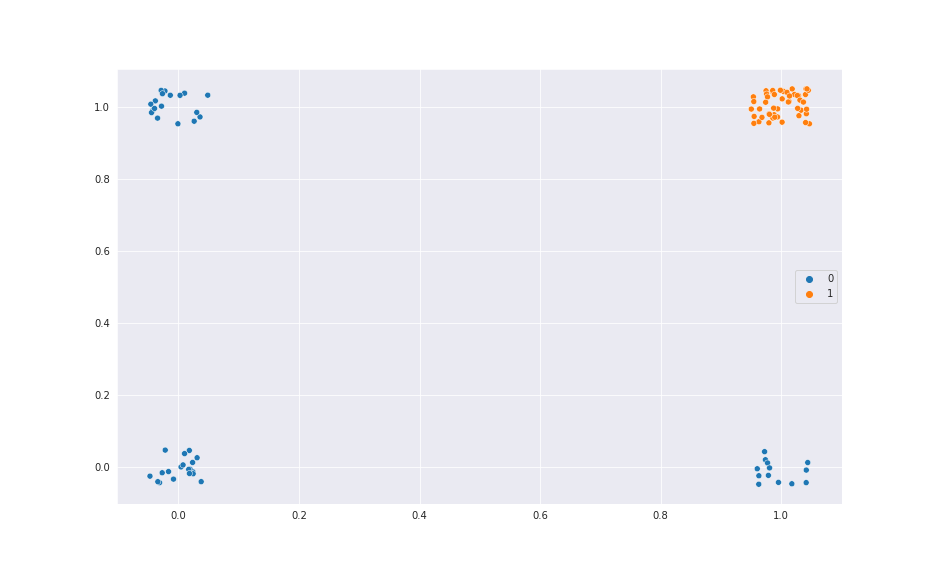
\includegraphics[width=0.7\textwidth]{images/01_data.png}
\end{figure}

\section{Badania}

\subsection{Metodyka badań}
Wszystkie eksperymenty powtórzono 20 razy dla każdej wartości badanego parametru.
Wyjątkiem jest badanie wpływu funkcji aktywacji, które wykonano 1000 razy, w celu
uzyskania bardziej miarodajnego wyniku. 

\subsection{Perceptron}
\label{headings}

\subsubsection{Próg $\theta$}
Próg $\theta$ jest ważnym parametrem, który znacząco wpływa na szybkość uczenia.
Zarówno zbyt mała, jak i za duża wartość $\theta$ wpływa negatywnie na proces optymalizacji.
Wartości z przedziału $\left[0.01, 1\right]$ pozwalają wytrenować algorytm w stosunkowo krótkim czasie.

\begin{figure}[h]
  \caption{Wpływ parametru $\theta$}
  \centering
    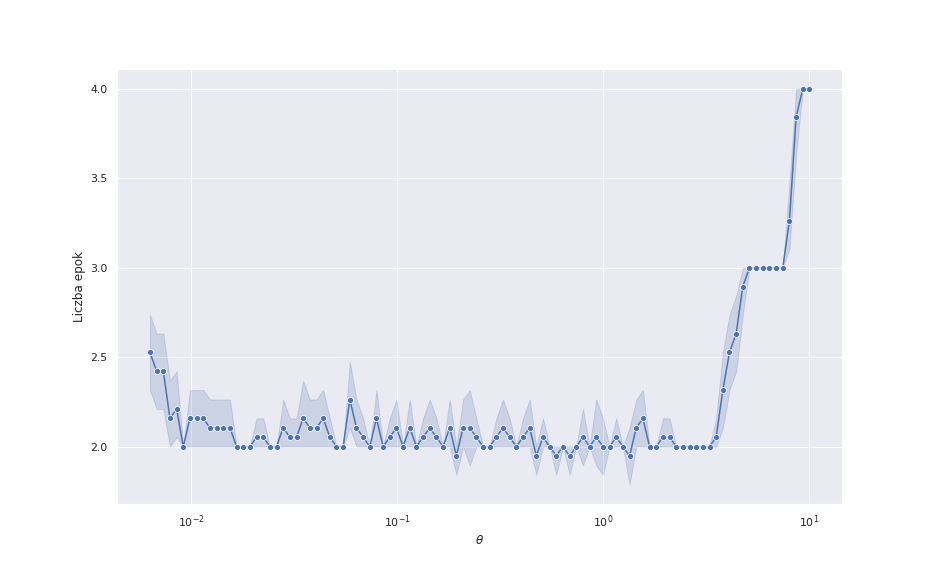
\includegraphics[width=0.7\textwidth]{images/02_per_theta.png}
\end{figure}

\subsubsection{Inicjalizacja wag}

Wagi zostały zainicjowane z rozkłądu jednostajnego.
Na krańce przedziałów wybrano liczby leżące w tej samej odległości od puntu zerowego.
Wartości z przedziału $\left(0, 1\right]$ zapewniają najszybsze uczenie modelu.

\begin{figure}[h]
  \caption{Wpływ inicjalizacji wag}
  \centering
    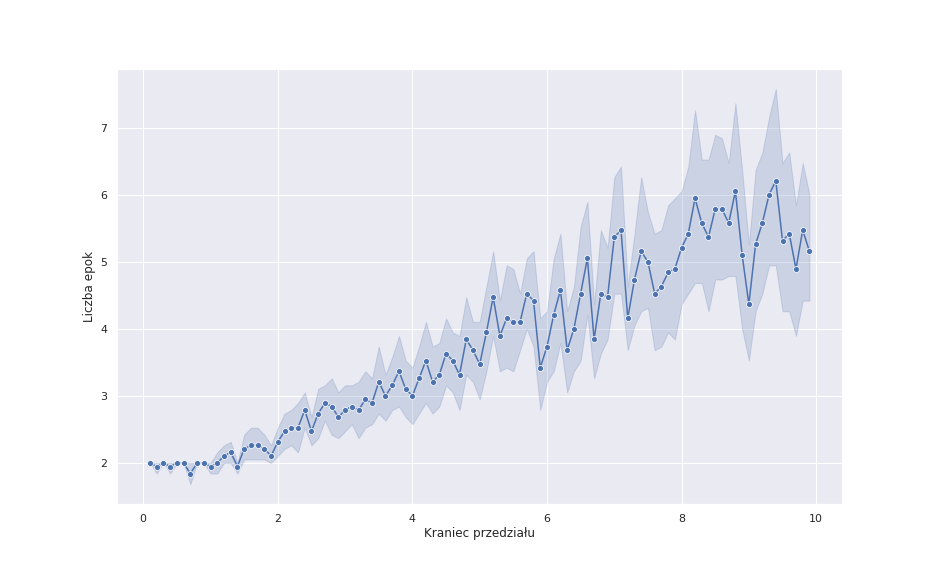
\includegraphics[width=0.7\textwidth]{images/03_per_interval.png}
\end{figure}

\subsubsection{Współczynnik uczenia $\alpha$}
Hiperparametr $\alpha$ naturalnie wpływa na szybkość uczenia.
Zbyt małe wartości tego współczynnika skutkowały bardzo wolnym zbieganiem do optimum.
Co ciekawe, liczba epok pozostawała względnie stała dla większych wartości $\alpha$

\begin{figure}[h]
  \caption{Wpływ $\alpha$ }
  \centering
    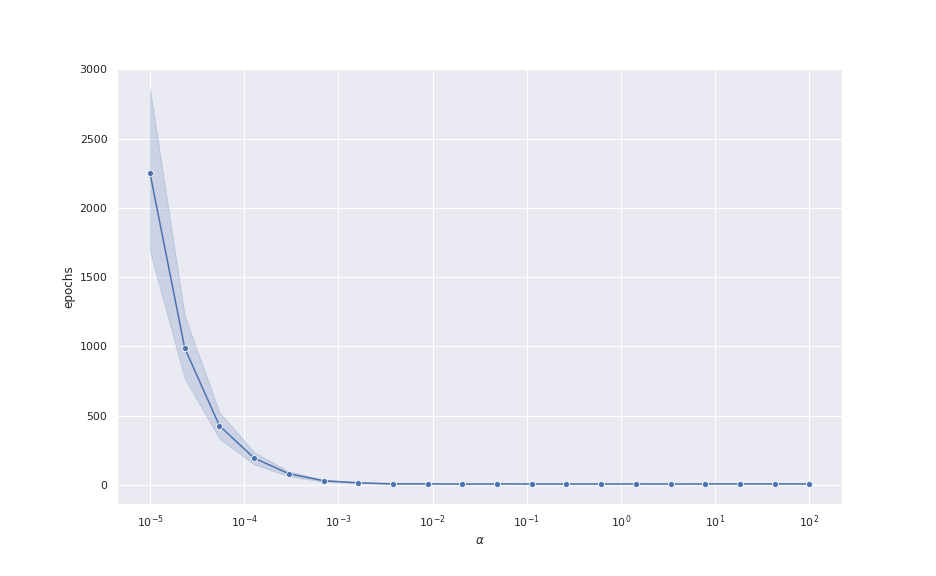
\includegraphics[width=0.7\textwidth]{images/04_per_lr.png}
\end{figure}

\subsubsection{Porównanie funkcji aktywacji}
Różnica między funkcją unipolarną a bipolarną nie wydaje się być znacząca.
Średnia liczba epok treningowych jest bardzo zbliżona.
Dla funkcji bipolarnej wyniki są bardziej skupione wokół średniej.
W celu uzyskania dokłądniejszych wyników badanie powtórzono 1000 razy.

\begin{figure}[h]
  \caption{Porównanie funkcji unipolarnej i bipolarnej}
  \centering
    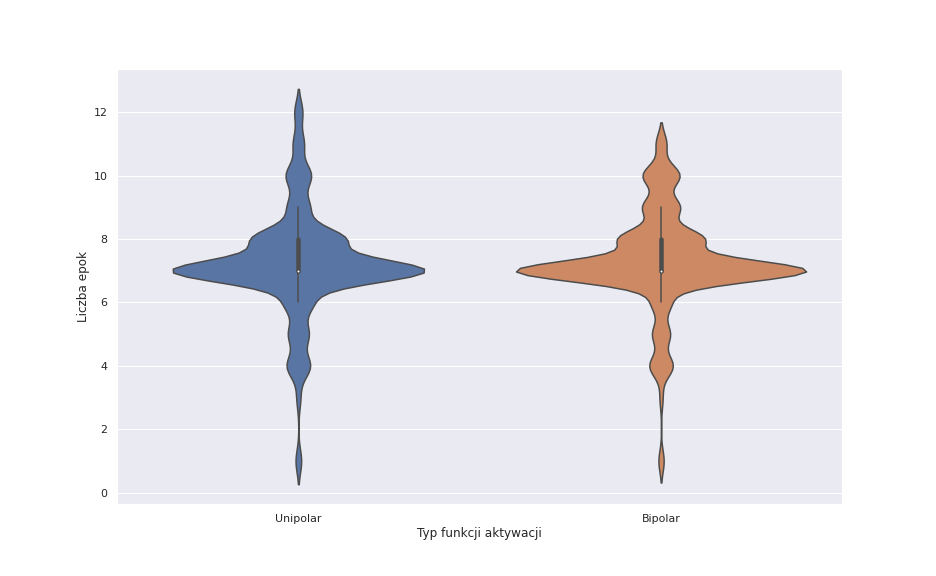
\includegraphics[width=1\textwidth]{images/05_per_uni_bi.png}
\end{figure}


\subsection {Adaline}

\subsubsection{Inicjalizacja wag}
Podobnie jak w przypadku Perceptronu, wagi zostały zainicjowane z rozkładu jednostajnego.
Algorytm Adaline jest bardziej podatny na skalę wag dobraną podczas inicjalizacji.
W przypadku wag z przedziału $\left(0, 0.25\right]$ potrzeba było zaledwie jednej
epoki do osiągnięcia optimum z zadaną dokładnością.

\begin{figure}[h]
  \caption{Wpływ inicjalizacji wag}
  \centering
    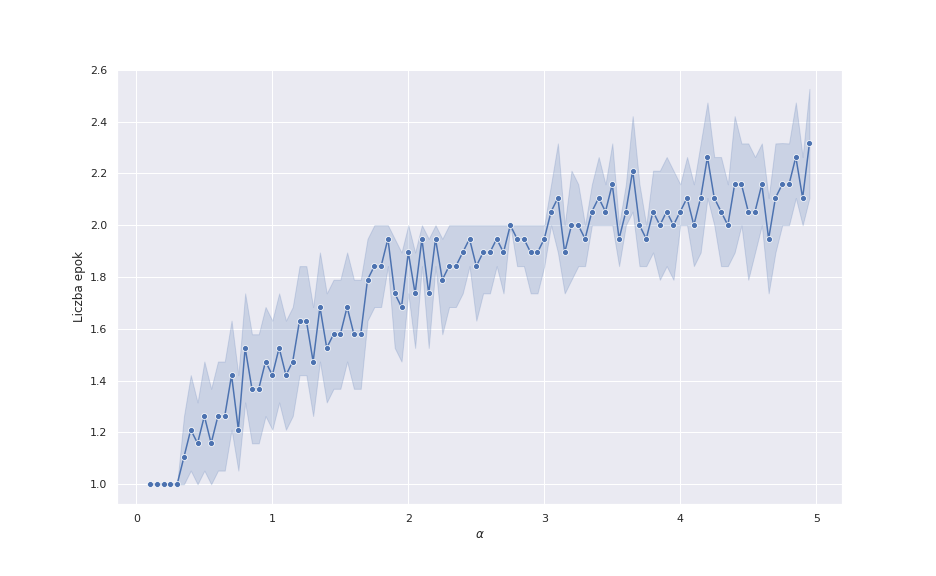
\includegraphics[width=0.7\textwidth]{images/06_ada_interval.png}
\end{figure}


\subsubsection{Współczynnik uczenia $\mu$}
Wpływ współczynnika uczenia okazał się znaczący.
Zbyt małe wartości były powodem wolnego zbiegania do optimum.
Zachowanie funkcji okazało się szczególnie interesujące dla dużych wartości $\mu$.
Ustawienie współczynnika uczenia większego od 0.01 spowodowało eksplozję gradientów, która uniemożliwiła poprawną optymalizację.
Problem zanikających lub eksplodujących gradientów dotyczy szczególnie głębokich sieci neuronowych.
Rozwiązaniem jest dobór odpowiedniej wartości $\mu$ oraz specjalne metody inicjalizacji wag.


\begin{figure}[h]
  \caption{Wpływ $\mu$}
  \centering
    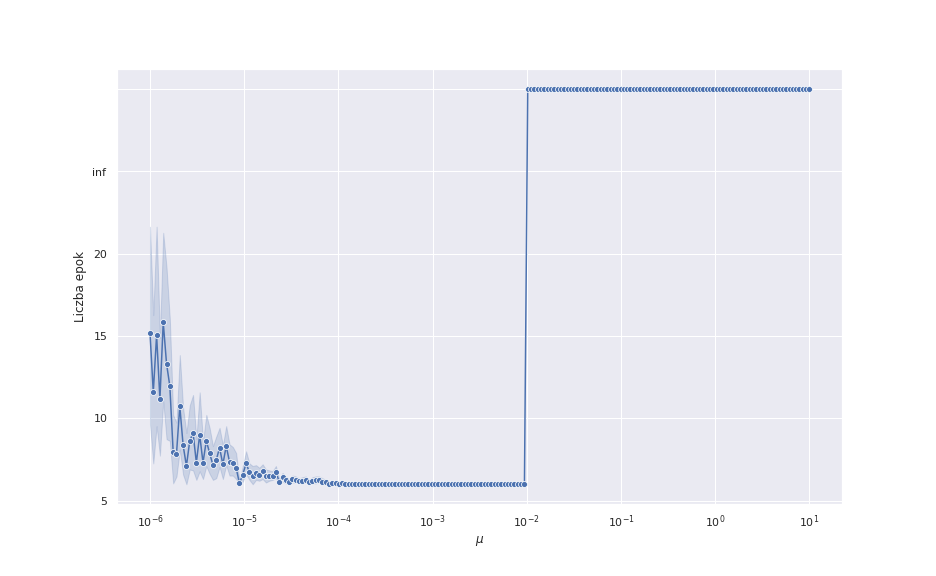
\includegraphics[width=0.7\textwidth]{images/07_ada_lr.png}
\end{figure}


All tables must be centered, neat, clean and legible.  The table
number and title always appear before the table.  See
Table~\ref{sample-table}.

Place one line space before the table title, one line space after the
table title, and one line space after the table. The table title must
be lower case (except for first word and proper nouns); tables are
numbered consecutively.

Note that publication-quality tables \emph{do not contain vertical
  rules.} We strongly suggest the use of the \verb+booktabs+ package,
which allows for typesetting high-quality, professional tables:
\begin{center}
  \url{https://www.ctan.org/pkg/booktabs}
\end{center}
This package was used to typeset Table~\ref{sample-table}.

\begin{table}[t]
  \caption{Sample table title}
  \label{sample-table}
  \centering
  \begin{tabular}{lll}
    \toprule
    \multicolumn{2}{c}{Part}                   \\
    \cmidrule{1-2}
    Name     & Description     & Size ($\mu$m) \\
    \midrule
    Dendrite & Input terminal  & $\sim$100     \\
    Axon     & Output terminal & $\sim$10      \\
    Soma     & Cell body       & up to $10^6$  \\
    \bottomrule
  \end{tabular}
\end{table}

\section{Final instructions}

Do not change any aspects of the formatting parameters in the style
files.  In particular, do not modify the width or length of the
rectangle the text should fit into, and do not change font sizes
(except perhaps in the \textbf{References} section; see below). Please
note that pages should be numbered.

\section{Preparing PDF files}

Please prepare submission files with paper size ``US Letter,'' and
not, for example, ``A4.''

Fonts were the main cause of problems in the past years. Your PDF file
must only contain Type 1 or Embedded TrueType fonts. Here are a few
instructions to achieve this.

\begin{itemize}

\item You should directly generate PDF files using \verb+pdflatex+.

\item You can check which fonts a PDF files uses.  In Acrobat Reader,
  select the menu Files$>$Document Properties$>$Fonts and select Show
  All Fonts. You can also use the program \verb+pdffonts+ which comes
  with \verb+xpdf+ and is available out-of-the-box on most Linux
  machines.

\item The IEEE has recommendations for generating PDF files whose
  fonts are also acceptable for NIPS. Please see
  \url{http://www.emfield.org/icuwb2010/downloads/IEEE-PDF-SpecV32.pdf}

\item \verb+xfig+ "patterned" shapes are implemented with bitmap
  fonts.  Use "solid" shapes instead.

\item The \verb+\bbold+ package almost always uses bitmap fonts.  You
  should use the equivalent AMS Fonts:
\begin{verbatim}
   \usepackage{amsfonts}
\end{verbatim}
followed by, e.g., \verb+\mathbb{R}+, \verb+\mathbb{N}+, or
\verb+\mathbb{C}+ for $\mathbb{R}$, $\mathbb{N}$ or $\mathbb{C}$.  You
can also use the following workaround for reals, natural and complex:
\begin{verbatim}
   \newcommand{\RR}{I\!\!R} %real numbers
   \newcommand{\Nat}{I\!\!N} %natural numbers
   \newcommand{\CC}{I\!\!\!\!C} %complex numbers
\end{verbatim}
Note that \verb+amsfonts+ is automatically loaded by the
\verb+amssymb+ package.

\end{itemize}

If your file contains type 3 fonts or non embedded TrueType fonts, we
will ask you to fix it.

\subsection{Margins in \LaTeX{}}

Most of the margin problems come from figures positioned by hand using
\verb+\special+ or other commands. We suggest using the command
\verb+\includegraphics+ from the \verb+graphicx+ package. Always
specify the figure width as a multiple of the line width as in the
example below:
\begin{verbatim}
   \usepackage[pdftex]{graphicx} ...
   \includegraphics[width=0.8\linewidth]{myfile.pdf}
\end{verbatim}
See Section 4.4 in the graphics bundle documentation
(\url{http://mirrors.ctan.org/macros/latex/required/graphics/grfguide.pdf})

A number of width problems arise when \LaTeX{} cannot properly
hyphenate a line. Please give LaTeX hyphenation hints using the
\verb+\-+ command when necessary.

\subsubsection*{Acknowledgments}

Use unnumbered third level headings for the acknowledgments. All
acknowledgments go at the end of the paper. Do not include
acknowledgments in the anonymized submission, only in the final paper.

\section*{References}

References follow the acknowledgments. Use unnumbered first-level
heading for the references. Any choice of citation style is acceptable
as long as you are consistent. It is permissible to reduce the font
size to \verb+small+ (9 point) when listing the references. {\bf
  Remember that you can go over 8 pages as long as the subsequent ones contain
  \emph{only} cited references.}
\medskip

\small

[1] Alexander, J.A.\ \& Mozer, M.C.\ (1995) Template-based algorithms
for connectionist rule extraction. In G.\ Tesauro, D.S.\ Touretzky and
T.K.\ Leen (eds.), {\it Advances in Neural Information Processing
  Systems 7}, pp.\ 609--616. Cambridge, MA: MIT Press.

[2] Bower, J.M.\ \& Beeman, D.\ (1995) {\it The Book of GENESIS:
  Exploring Realistic Neural Models with the GEneral NEural SImulation
  System.}  New York: TELOS/Springer--Verlag.

[3] Hasselmo, M.E., Schnell, E.\ \& Barkai, E.\ (1995) Dynamics of
learning and recall at excitatory recurrent synapses and cholinergic
modulation in rat hippocampal region CA3. {\it Journal of
  Neuroscience} {\bf 15}(7):5249-5262.

\end{document}

Poni¿ej znajduje siê tabela, w której znajduj¹ siê informacje jak zapisaæ poprawnie polskie znaki w formie zakodowanej:
POLSKA LITERA   KOD TEX POLSKA LITERA   KOD TEX
¹       \k{a}   ¥       \k{A}
æ       \'c     Æ       \'C
ê       \k{e}   Ê       \k{E}
³       \l{}    £       \L{}
ñ       \'n     Ñ       \'N
ó       \'o     Ó       \'O
œ       \'s     Œ       \'S
¿       \.z     ¯       \.Z
Ÿ       \'z            \'Z

